\chapter{Aplikacja rozwiązująca problem przydziału kwadratowego z wykorzystaniem kwantowego algorytmu ewolucyjnego}
\label{cha:aplikacja}
Jak już zostało to nadmienione parokrotnie wcześniej, jednym z celów realizowanej pracy dyplomowej było napisanie aplikacji, która przy wykorzystaniu jednego z algorytmów aproksymacyjnych będzie rozwiązywać problem przydziału kwadratowego. Wybór padł na kwantowy algorytm ewolucyjny NPQGA opisany w rozdziale czwartym. Uwzględnione w nim zmiany oraz modyfikacje zostały przedstawione w piątym rozdziale. Program został zrealizowany jako aplikacja konsolowa i napisana w języku C\#. O tym, że aplikacja będzie konsolowa zadecydował fakt, iż jej celem nadrzędnym jest znajdywanie rozwiązania problemu QAP i ma służyć jako narzędzie pozwalające zweryfikować działanie algorytmu. Aspekty wizualne są jedynie dodatkiem, który nie wpływa na jakość rozwiązania problemu.

\section{Interfejsy klas}
Punktem wyjścia do rozpoczęcia prac był zestaw interfejsów klas przygotowanych przez opiekuna niniejszej pracy. Interfejs klasy w sensie języka C\# jest narzędziem wykorzystywanym w technice dziedziczenia i określa metody i właściwości jakie klasa dziedzicząca po nim musi implementować. Jednakże ciała metod nie są określone i zależą wyłącznie od implementacji w danej klasie. W przeciwieństwie do dziedziczeniu po klasach, istnieje możliwość dziedziczenia po wielu interfejsach. Dzięki wykorzystaniu interfejsów, napisane na potrzeby pracy klasy będzie można wykorzystać w innych aplikacjach, czy to już istniejących, ale i w tych, które dopiero powstaną. Poniżej znajduje się lista interfejsów, które należało zaimplementować:
\begin{enumerate}
\item IEvolutionAlgorithm,
\item IOptimisationAlgorithm,
\item IPopulation,
\item ISolution,
\item IEvolutionaryOperator,
\item IMutationOperator,
\item ICrossoverOperator.
\end{enumerate}

Pierwszy interfejs \textit{IEvolutionAlgorithm} określa, co klasy reprezentujące dowolny algorytm ewolucyjny powinny implementować. Następnie interfejs \textit{IOptimisationAlgorithm} służy do reprezentowania ogólnego algorytmu optymalizacji, nie tylko ewolucyjnego i  interfejs nr 1 dziedziczy po nim. Klasa, której obiekty przedstawiają rozwiązania problemu dziedziczy po interfejsie \textit{ISolution}, a cała populacja rozwiązań po \textit{IPopulation}. Klasy mające za zadanie reprezentować operatory ewolucyjne dziedziczą po interfejsie \textit{IEvolutionaryOperator} i należą do nich klasy odpowiadające za przedstawianie operatorów mutacji i krzyżowania, które z kolei muszą dziedziczyć po interfejsach \textit{IMutationOperator} i \textit{ICrossoverOperator}.

\section{Struktura danych}
By algorytm mógł znaleźć rozwiązanie problemu, musi przetwarzać całą populację rozwiązań. Dlatego też została napisana klasa \textit{Population}, dziedzicząca po interfejsie \textit{IPopulation}. Populacja natomiast zawiera w sobie listę osobników, rozwiązań, które reprezentowane są przez obiekty klasy \textit{Solution} dziedziczącej z kolei po interfejsie \textit{ISolution}. Postacią rozwiązania w problemie przydziału kwadratowego jest permutacja, określająca, który obiekt został przypisany do kolejnych lokalizacji. Z tego powodu obiekty klasy \textit{Solution} zawierają w sobie listę obiektów reprezentujących elementy permutacji. Klasa tych obiektów została nazwana \textit{Chromosome}. Należy tutaj wyjaśnić pewną nieścisłość w terminach używanych w algorytmach genetycznych. \textit{Chromosomami} zwykło się nazywać kompletne rozwiązania, a ich fragmenty kodujące rozwiązanie \textit{genami}. Z racji, iż w aplikacji rozwiązania problemu reprezentowane są przez obiekty klasy \textit{Solution}, a element permutacji nie jest najmniejsza porcją informacji, postanowiono nazwać te porcje chromosomami, a ich najmniejszą część \textit{genem}. A więc \textit{chromosomy} składają się z kubitów reprezentowanych przez klasę \textit{Qbit}. Poprzez zdekodowanie stanu kubitów określa się wartość chromosomu, a następnie poprzez omówioną w rozdziale czwartym konwersję otrzymuje się permutacyjną postać rozwiązania problemu QAP.
\newpage
\begin{figure}[!t]
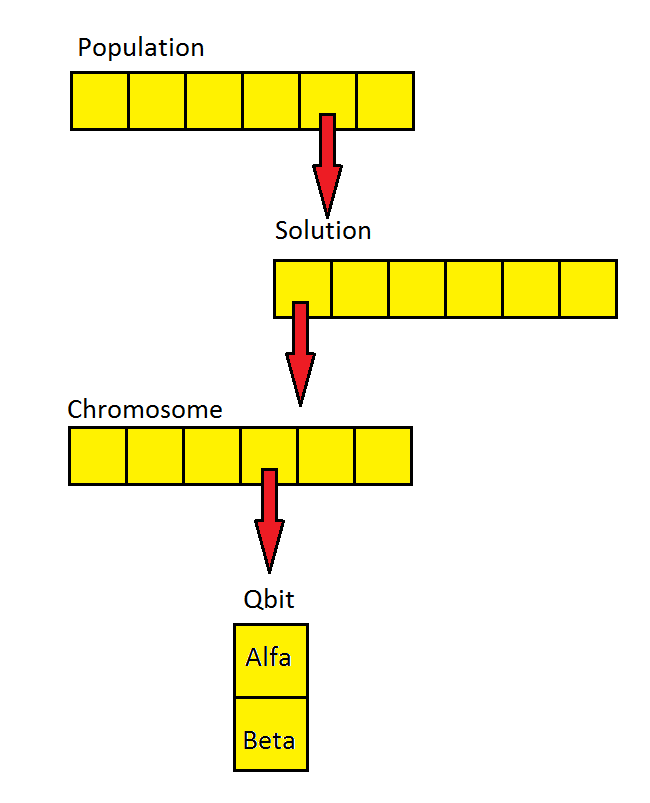
\includegraphics[scale=0.4]{data_structure}
\caption{Struktura danych}
\end{figure}

W kontekście struktury danych należy jeszcze wspomnieć o macierzach przepływu i odległości problemu QAP. Ich wartości są wczytywane z plików \textit{.dat} zawierających rozmiar problemu oraz odpowiednio macierze odległości i przepływu i są następnie trzymane w obiekcie klasy \textit{QapData} zrealizowanej jako singleton, czyli jako specjalna klasa o globalnym dostępnie pozwalająca na utworzenie tylko jednego jej obiektu. Posiada ona także mechanizmy, które bez wiedzy użytkownika same dbają o to, by faktycznie istniał jeden jej obiekt i jej instancja została utworzona podczas pierwszej próby jej użycia.

\section{Interfejs użytkownika}
Po uruchomieniu aplikacji użytkownik ma możliwość ustawienia kilku parametrów algorytmu. Należą do nich:
\begin{itemize}
\item minimalne i maksymalne prawdopodobieństwo krzyżowania,
\item prawdopodobieństwo mutacji,
\item metoda selekcji,
\item metoda krzyżowania,
\item rozmiar populacji,
\item ilość iteracji algorytmu,
\item testowy zestaw danych.
\end{itemize}

W przypadku operatora selekcji do wyboru są dwie metody: ruletkowa oraz rankingowa. Spośród metod krzyżowania dostępne są trzy opcje: CX, OX i PMX. Sposoby działania wymienionych operatorów selekcji i krzyżowania zostały omówione we wcześniejszych rozdziałach.

\section{Rezultaty działania aplikacji}
Po wykonaniu wszystkich iteracji algorytmu, program zwraca najlepsze znalezione rozwiązanie wraz z wartością funkcji celu oraz informację o tym, w której iteracji zostało zwrócone rozwiązanie. Program po każdym zakończeniu działania algorytmu tworzy także plik, o podanej przez użytkownika nazwie, zawierający informacje o najlepszym i najgorszym rozwiązaniu w każdej iteracji, wartości ich funkcji celu i permutacje odpowiadające tym rozwiązaniom, a także średnią wartość funkcji celu w każdej z iteracji i ustawione przez użytkownika parametry algorytmu. Dane zawarte w tych plikach pozwalają na porównywanie działania algorytmów dla różnych ustawień, sprawdzenia dla których parametrów uzyskiwane są lepsze bądź gorsze wyniki.